\documentclass[1p]{elsarticle_modified}
%\bibliographystyle{elsarticle-num}

%\usepackage[colorlinks]{hyperref}
%\usepackage{abbrmath_seonhwa} %\Abb, \Ascr, \Acal ,\Abf, \Afrak
\usepackage{amsfonts}
\usepackage{amssymb}
\usepackage{amsmath}
\usepackage{amsthm}
\usepackage{scalefnt}
\usepackage{amsbsy}
\usepackage{kotex}
\usepackage{caption}
\usepackage{subfig}
\usepackage{color}
\usepackage{graphicx}
\usepackage{xcolor} %% white, black, red, green, blue, cyan, magenta, yellow
\usepackage{float}
\usepackage{setspace}
\usepackage{hyperref}

\usepackage{tikz}
\usetikzlibrary{arrows}

\usepackage{multirow}
\usepackage{array} % fixed length table
\usepackage{hhline}

%%%%%%%%%%%%%%%%%%%%%
\makeatletter
\renewcommand*\env@matrix[1][\arraystretch]{%
	\edef\arraystretch{#1}%
	\hskip -\arraycolsep
	\let\@ifnextchar\new@ifnextchar
	\array{*\c@MaxMatrixCols c}}
\makeatother %https://tex.stackexchange.com/questions/14071/how-can-i-increase-the-line-spacing-in-a-matrix
%%%%%%%%%%%%%%%

\usepackage[normalem]{ulem}

\newcommand{\msout}[1]{\ifmmode\text{\sout{\ensuremath{#1}}}\else\sout{#1}\fi}
%SOURCE: \msout is \stkout macro in https://tex.stackexchange.com/questions/20609/strikeout-in-math-mode

\newcommand{\cancel}[1]{
	\ifmmode
	{\color{red}\msout{#1}}
	\else
	{\color{red}\sout{#1}}
	\fi
}

\newcommand{\add}[1]{
	{\color{blue}\uwave{#1}}
}

\newcommand{\replace}[2]{
	\ifmmode
	{\color{red}\msout{#1}}{\color{blue}\uwave{#2}}
	\else
	{\color{red}\sout{#1}}{\color{blue}\uwave{#2}}
	\fi
}

\newcommand{\Sol}{\mathcal{S}} %segment
\newcommand{\D}{D} %diagram
\newcommand{\A}{\mathcal{A}} %arc


%%%%%%%%%%%%%%%%%%%%%%%%%%%%%5 test

\def\sl{\operatorname{\textup{SL}}(2,\Cbb)}
\def\psl{\operatorname{\textup{PSL}}(2,\Cbb)}
\def\quan{\mkern 1mu \triangleright \mkern 1mu}

\theoremstyle{definition}
\newtheorem{thm}{Theorem}[section]
\newtheorem{prop}[thm]{Proposition}
\newtheorem{lem}[thm]{Lemma}
\newtheorem{ques}[thm]{Question}
\newtheorem{cor}[thm]{Corollary}
\newtheorem{defn}[thm]{Definition}
\newtheorem{exam}[thm]{Example}
\newtheorem{rmk}[thm]{Remark}
\newtheorem{alg}[thm]{Algorithm}

\newcommand{\I}{\sqrt{-1}}
\begin{document}

%\begin{frontmatter}
%
%\title{Boundary parabolic representations of knots up to 8 crossings}
%
%%% Group authors per affiliation:
%\author{Yunhi Cho} 
%\address{Department of Mathematics, University of Seoul, Seoul, Korea}
%\ead{yhcho@uos.ac.kr}
%
%
%\author{Seonhwa Kim} %\fnref{s_kim}}
%\address{Center for Geometry and Physics, Institute for Basic Science, Pohang, 37673, Korea}
%\ead{ryeona17@ibs.re.kr}
%
%\author{Hyuk Kim}
%\address{Department of Mathematical Sciences, Seoul National University, Seoul 08826, Korea}
%\ead{hyukkim@snu.ac.kr}
%
%\author{Seokbeom Yoon}
%\address{Department of Mathematical Sciences, Seoul National University, Seoul, 08826,  Korea}
%\ead{sbyoon15@snu.ac.kr}
%
%\begin{abstract}
%We find all boundary parabolic representation of knots up to 8 crossings.
%
%\end{abstract}
%\begin{keyword}
%    \MSC[2010] 57M25 
%\end{keyword}
%
%\end{frontmatter}

%\linenumbers
%\tableofcontents
%
\newcommand\colored[1]{\textcolor{white}{\rule[-0.35ex]{0.8em}{1.4ex}}\kern-0.8em\color{red} #1}%
%\newcommand\colored[1]{\textcolor{white}{ #1}\kern-2.17ex	\textcolor{white}{ #1}\kern-1.81ex	\textcolor{white}{ #1}\kern-2.15ex\color{red}#1	}

{\Large $\underline{12n_{0662}~(K12n_{0662})}$}

\setlength{\tabcolsep}{10pt}
\renewcommand{\arraystretch}{1.6}
\vspace{1cm}\begin{tabular}{m{100pt}>{\centering\arraybackslash}m{274pt}}
\multirow{5}{120pt}{
	\centering
	\includegraphics[width=112pt]{../../../GIT/diagram.site/Diagrams/png/2751_12n_0662.png}\\
\ \ \ A knot diagram\footnotemark}&
\allowdisplaybreaks
\textbf{Linearized knot diagam} \\
\cline{2-2}
 &
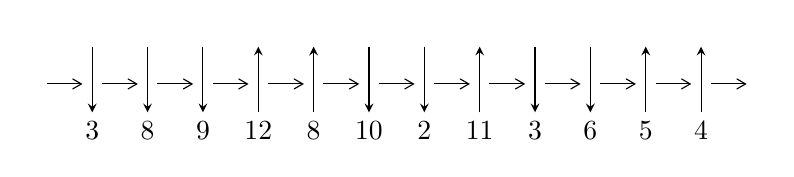
\begin{tikzpicture}[x=20pt, y=17pt]
	% nodes
	\node (C0) at (0, 0) {};
	\node (C1) at (1, 0) {};
	\node (C1U) at (1, +1) {};
	\node (C1D) at (1, -1) {3};

	\node (C2) at (2, 0) {};
	\node (C2U) at (2, +1) {};
	\node (C2D) at (2, -1) {8};

	\node (C3) at (3, 0) {};
	\node (C3U) at (3, +1) {};
	\node (C3D) at (3, -1) {9};

	\node (C4) at (4, 0) {};
	\node (C4U) at (4, +1) {};
	\node (C4D) at (4, -1) {12};

	\node (C5) at (5, 0) {};
	\node (C5U) at (5, +1) {};
	\node (C5D) at (5, -1) {8};

	\node (C6) at (6, 0) {};
	\node (C6U) at (6, +1) {};
	\node (C6D) at (6, -1) {10};

	\node (C7) at (7, 0) {};
	\node (C7U) at (7, +1) {};
	\node (C7D) at (7, -1) {2};

	\node (C8) at (8, 0) {};
	\node (C8U) at (8, +1) {};
	\node (C8D) at (8, -1) {11};

	\node (C9) at (9, 0) {};
	\node (C9U) at (9, +1) {};
	\node (C9D) at (9, -1) {3};

	\node (C10) at (10, 0) {};
	\node (C10U) at (10, +1) {};
	\node (C10D) at (10, -1) {6};

	\node (C11) at (11, 0) {};
	\node (C11U) at (11, +1) {};
	\node (C11D) at (11, -1) {5};

	\node (C12) at (12, 0) {};
	\node (C12U) at (12, +1) {};
	\node (C12D) at (12, -1) {4};
	\node (C13) at (13, 0) {};

	% arrows
	\draw[->,>={angle 60}]
	(C0) edge (C1) (C1) edge (C2) (C2) edge (C3) (C3) edge (C4) (C4) edge (C5) (C5) edge (C6) (C6) edge (C7) (C7) edge (C8) (C8) edge (C9) (C9) edge (C10) (C10) edge (C11) (C11) edge (C12) (C12) edge (C13) ;	\draw[->,>=stealth]
	(C1U) edge (C1D) (C2U) edge (C2D) (C3U) edge (C3D) (C4D) edge (C4U) (C5D) edge (C5U) (C6U) edge (C6D) (C7U) edge (C7D) (C8D) edge (C8U) (C9U) edge (C9D) (C10U) edge (C10D) (C11D) edge (C11U) (C12D) edge (C12U) ;
	\end{tikzpicture} \\
\hhline{~~} \\& 
\textbf{Solving Sequence} \\ \cline{2-2} 
 &
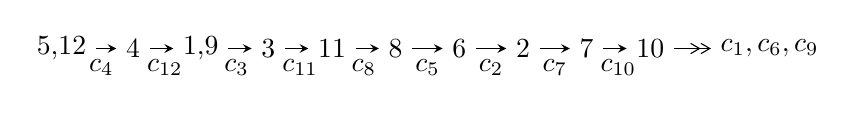
\begin{tikzpicture}[x=23pt, y=7pt]
	% node
	\node (A0) at (-1/8, 0) {5,12};
	\node (A1) at (1, 0) {4};
	\node (A2) at (33/16, 0) {1,9};
	\node (A3) at (25/8, 0) {3};
	\node (A4) at (33/8, 0) {11};
	\node (A5) at (41/8, 0) {8};
	\node (A6) at (49/8, 0) {6};
	\node (A7) at (57/8, 0) {2};
	\node (A8) at (65/8, 0) {7};
	\node (A9) at (73/8, 0) {10};
	\node (C1) at (1/2, -1) {$c_{4}$};
	\node (C2) at (3/2, -1) {$c_{12}$};
	\node (C3) at (21/8, -1) {$c_{3}$};
	\node (C4) at (29/8, -1) {$c_{11}$};
	\node (C5) at (37/8, -1) {$c_{8}$};
	\node (C6) at (45/8, -1) {$c_{5}$};
	\node (C7) at (53/8, -1) {$c_{2}$};
	\node (C8) at (61/8, -1) {$c_{7}$};
	\node (C9) at (69/8, -1) {$c_{10}$};
	\node (A10) at (11, 0) {$c_{1},c_{6},c_{9}$};

	% edge
	\draw[->,>=stealth]	
	(A0) edge (A1) (A1) edge (A2) (A2) edge (A3) (A3) edge (A4) (A4) edge (A5) (A5) edge (A6) (A6) edge (A7) (A7) edge (A8) (A8) edge (A9) ;
	\draw[->>,>={angle 60}]	
	(A9) edge (A10);
\end{tikzpicture} \\ 

\end{tabular} \\

\footnotetext{
The image of knot diagram is generated by the software ``\textbf{Draw programme}" developed by Andrew Bartholomew(\url{http://www.layer8.co.uk/maths/draw/index.htm\#Running-draw}), where we modified some parts for our purpose(\url{https://github.com/CATsTAILs/LinksPainter}).
}\phantom \\ \newline 
\centering \textbf{Ideals for irreducible components\footnotemark of $X_{\text{par}}$} 
 
\begin{align*}
I^u_{1}&=\langle 
3.56429\times10^{66} u^{46}+1.38822\times10^{67} u^{45}+\cdots+1.35802\times10^{68} b-1.96080\times10^{67},\\
\phantom{I^u_{1}}&\phantom{= \langle  }-2.47131\times10^{68} u^{46}-9.94693\times10^{68} u^{45}+\cdots+1.49382\times10^{69} a+2.99067\times10^{69},\;u^{47}+4 u^{46}+\cdots+u+11\rangle \\
I^u_{2}&=\langle 
-4 u^{16}+4 u^{15}+\cdots+b-4,\;-2 u^{17}+2 u^{16}+\cdots+a-4,\;u^{18}- u^{17}+\cdots-4 u+1\rangle \\
\\
\end{align*}
\raggedright * 2 irreducible components of $\dim_{\mathbb{C}}=0$, with total 65 representations.\\
\footnotetext{All coefficients of polynomials are rational numbers. But the coefficients are sometimes approximated in decimal forms when there is not enough margin.}
\newpage
\renewcommand{\arraystretch}{1}
\centering \section*{I. $I^u_{1}= \langle 3.56\times10^{66} u^{46}+1.39\times10^{67} u^{45}+\cdots+1.36\times10^{68} b-1.96\times10^{67},\;-2.47\times10^{68} u^{46}-9.95\times10^{68} u^{45}+\cdots+1.49\times10^{69} a+2.99\times10^{69},\;u^{47}+4 u^{46}+\cdots+u+11 \rangle$}
\flushleft \textbf{(i) Arc colorings}\\
\begin{tabular}{m{7pt} m{180pt} m{7pt} m{180pt} }
\flushright $a_{5}=$&$\begin{pmatrix}1\\0\end{pmatrix}$ \\
\flushright $a_{12}=$&$\begin{pmatrix}0\\u\end{pmatrix}$ \\
\flushright $a_{4}=$&$\begin{pmatrix}1\\u^2\end{pmatrix}$ \\
\flushright $a_{1}=$&$\begin{pmatrix}u\\u^3+u\end{pmatrix}$ \\
\flushright $a_{9}=$&$\begin{pmatrix}0.165436 u^{46}+0.665872 u^{45}+\cdots+47.6506 u-2.00203\\-0.0262463 u^{46}-0.102224 u^{45}+\cdots+2.75590 u+0.144387\end{pmatrix}$ \\
\flushright $a_{3}=$&$\begin{pmatrix}0.0228210 u^{46}+0.0919063 u^{45}+\cdots+22.9291 u+6.98832\\-0.0353642 u^{46}-0.136035 u^{45}+\cdots-1.25538 u+0.587575\end{pmatrix}$ \\
\flushright $a_{11}=$&$\begin{pmatrix}- u\\u\end{pmatrix}$ \\
\flushright $a_{8}=$&$\begin{pmatrix}0.172179 u^{46}+0.702253 u^{45}+\cdots+49.1886 u-1.92623\\-0.0329894 u^{46}-0.138604 u^{45}+\cdots+1.21792 u+0.0685910\end{pmatrix}$ \\
\flushright $a_{6}=$&$\begin{pmatrix}-0.0344253 u^{46}-0.174526 u^{45}+\cdots+8.78426 u+2.63038\\-0.0166373 u^{46}-0.0395220 u^{45}+\cdots-0.358128 u+0.921788\end{pmatrix}$ \\
\flushright $a_{2}=$&$\begin{pmatrix}-0.0320584 u^{46}-0.155060 u^{45}+\cdots-31.9101 u+3.00707\\-0.0833370 u^{46}-0.330300 u^{45}+\cdots-4.63638 u+0.105685\end{pmatrix}$ \\
\flushright $a_{7}=$&$\begin{pmatrix}-0.0658054 u^{46}-0.226720 u^{45}+\cdots-5.52898 u-1.15248\\0.0661854 u^{46}+0.269634 u^{45}+\cdots+2.54666 u+0.0845939\end{pmatrix}$ \\
\flushright $a_{10}=$&$\begin{pmatrix}0.103828 u^{46}+0.400441 u^{45}+\cdots+14.9287 u-1.57199\\-0.0711995 u^{46}-0.276077 u^{45}+\cdots-0.849870 u+0.420108\end{pmatrix}$\\&\end{tabular}
\flushleft \textbf{(ii) Obstruction class $= -1$}\\~\\
\flushleft \textbf{(iii) Cusp Shapes $= -0.0933045 u^{46}-0.348811 u^{45}+\cdots+5.64696 u+9.13255$}\\~\\
\newpage\renewcommand{\arraystretch}{1}
\flushleft \textbf{(iv) u-Polynomials at the component}\newline \\
\begin{tabular}{m{50pt}|m{274pt}}
Crossings & \hspace{64pt}u-Polynomials at each crossing \\
\hline $$\begin{aligned}c_{1}\end{aligned}$$&$\begin{aligned}
&u^{47}+56 u^{46}+\cdots+13184125 u+534361
\end{aligned}$\\
\hline $$\begin{aligned}c_{2},c_{7}\end{aligned}$$&$\begin{aligned}
&u^{47}+2 u^{46}+\cdots-315 u+731
\end{aligned}$\\
\hline $$\begin{aligned}c_{3},c_{9}\end{aligned}$$&$\begin{aligned}
&u^{47}- u^{46}+\cdots-3782 u+667
\end{aligned}$\\
\hline $$\begin{aligned}c_{4},c_{11},c_{12}\end{aligned}$$&$\begin{aligned}
&u^{47}+4 u^{46}+\cdots+u+11
\end{aligned}$\\
\hline $$\begin{aligned}c_{5}\end{aligned}$$&$\begin{aligned}
&u^{47}+8 u^{46}+\cdots+151 u+149
\end{aligned}$\\
\hline $$\begin{aligned}c_{6},c_{10}\end{aligned}$$&$\begin{aligned}
&u^{47}+u^{46}+\cdots+368 u-103
\end{aligned}$\\
\hline $$\begin{aligned}c_{8}\end{aligned}$$&$\begin{aligned}
&u^{47}-4 u^{45}+\cdots+23 u+3
\end{aligned}$\\
\hline
\end{tabular}\\~\\
\newpage\renewcommand{\arraystretch}{1}
\flushleft \textbf{(v) Riley Polynomials at the component}\newline \\
\begin{tabular}{m{50pt}|m{274pt}}
Crossings & \hspace{64pt}Riley Polynomials at each crossing \\
\hline $$\begin{aligned}c_{1}\end{aligned}$$&$\begin{aligned}
&y^{47}-124 y^{46}+\cdots+5168548507345 y-285541678321
\end{aligned}$\\
\hline $$\begin{aligned}c_{2},c_{7}\end{aligned}$$&$\begin{aligned}
&y^{47}-56 y^{46}+\cdots+13184125 y-534361
\end{aligned}$\\
\hline $$\begin{aligned}c_{3},c_{9}\end{aligned}$$&$\begin{aligned}
&y^{47}-9 y^{46}+\cdots+9199640 y-444889
\end{aligned}$\\
\hline $$\begin{aligned}c_{4},c_{11},c_{12}\end{aligned}$$&$\begin{aligned}
&y^{47}+54 y^{46}+\cdots-10053 y-121
\end{aligned}$\\
\hline $$\begin{aligned}c_{5}\end{aligned}$$&$\begin{aligned}
&y^{47}+32 y^{46}+\cdots-1091719 y-22201
\end{aligned}$\\
\hline $$\begin{aligned}c_{6},c_{10}\end{aligned}$$&$\begin{aligned}
&y^{47}+5 y^{46}+\cdots+92988 y-10609
\end{aligned}$\\
\hline $$\begin{aligned}c_{8}\end{aligned}$$&$\begin{aligned}
&y^{47}-8 y^{46}+\cdots-113 y-9
\end{aligned}$\\
\hline
\end{tabular}\\~\\
\newpage\flushleft \textbf{(vi) Complex Volumes and Cusp Shapes}
$$\begin{array}{c|c|c}  
\text{Solutions to }I^u_{1}& \I (\text{vol} + \sqrt{-1}CS) & \text{Cusp shape}\\
 \hline 
\begin{aligned}
u &= \phantom{-}0.230731 + 1.086340 I \\
a &= \phantom{-}0.094144 - 1.313970 I \\
b &= \phantom{-}0.243008 + 0.226914 I\end{aligned}
 & \phantom{-}2.98236 + 2.61578 I & \phantom{-}1.41474 - 2.87187 I \\ \hline\begin{aligned}
u &= \phantom{-}0.230731 - 1.086340 I \\
a &= \phantom{-}0.094144 + 1.313970 I \\
b &= \phantom{-}0.243008 - 0.226914 I\end{aligned}
 & \phantom{-}2.98236 - 2.61578 I & \phantom{-}1.41474 + 2.87187 I \\ \hline\begin{aligned}
u &= \phantom{-}0.903444 + 0.695127 I \\
a &= \phantom{-}0.0854529 - 0.0543974 I \\
b &= \phantom{-}0.609527 + 0.047815 I\end{aligned}
 & \phantom{-}0.73075 + 3.15581 I & -8.86017 - 6.34037 I \\ \hline\begin{aligned}
u &= \phantom{-}0.903444 - 0.695127 I \\
a &= \phantom{-}0.0854529 + 0.0543974 I \\
b &= \phantom{-}0.609527 - 0.047815 I\end{aligned}
 & \phantom{-}0.73075 - 3.15581 I & -8.86017 + 6.34037 I \\ \hline\begin{aligned}
u &= -0.818444\phantom{ +0.000000I} \\
a &= \phantom{-}0.271814\phantom{ +0.000000I} \\
b &= -1.18073\phantom{ +0.000000I}\end{aligned}
 & -3.88729\phantom{ +0.000000I} & \phantom{-}1.39940\phantom{ +0.000000I} \\ \hline\begin{aligned}
u &= -0.315844 + 0.740860 I \\
a &= \phantom{-}0.67860 - 1.93996 I \\
b &= -0.053790 + 1.035250 I\end{aligned}
 & -7.17929 - 3.64393 I & -6.03198 + 2.78404 I \\ \hline\begin{aligned}
u &= -0.315844 - 0.740860 I \\
a &= \phantom{-}0.67860 + 1.93996 I \\
b &= -0.053790 - 1.035250 I\end{aligned}
 & -7.17929 + 3.64393 I & -6.03198 - 2.78404 I \\ \hline\begin{aligned}
u &= \phantom{-}0.660176 + 0.415759 I \\
a &= -0.815252 - 0.503616 I \\
b &= -0.269834 + 0.274621 I\end{aligned}
 & \phantom{-}0.54494 + 2.07931 I & -3.70506 - 3.58771 I \\ \hline\begin{aligned}
u &= \phantom{-}0.660176 - 0.415759 I \\
a &= -0.815252 + 0.503616 I \\
b &= -0.269834 - 0.274621 I\end{aligned}
 & \phantom{-}0.54494 - 2.07931 I & -3.70506 + 3.58771 I \\ \hline\begin{aligned}
u &= -0.259697 + 1.247040 I \\
a &= \phantom{-}1.70284 - 1.07261 I \\
b &= -1.80846 + 0.76841 I\end{aligned}
 & -7.62776 - 3.97997 I & \phantom{-0.000000 } 0\\
 \hline 
 \end{array}$$\newpage$$\begin{array}{c|c|c}  
\text{Solutions to }I^u_{1}& \I (\text{vol} + \sqrt{-1}CS) & \text{Cusp shape}\\
 \hline 
\begin{aligned}
u &= -0.259697 - 1.247040 I \\
a &= \phantom{-}1.70284 + 1.07261 I \\
b &= -1.80846 - 0.76841 I\end{aligned}
 & -7.62776 + 3.97997 I & \phantom{-0.000000 } 0 \\ \hline\begin{aligned}
u &= -1.048870 + 0.734928 I \\
a &= -0.199629 + 0.382583 I \\
b &= -0.707111 - 0.228325 I\end{aligned}
 & -6.81414 - 8.86603 I & \phantom{-0.000000 } 0 \\ \hline\begin{aligned}
u &= -1.048870 - 0.734928 I \\
a &= -0.199629 - 0.382583 I \\
b &= -0.707111 + 0.228325 I\end{aligned}
 & -6.81414 + 8.86603 I & \phantom{-0.000000 } 0 \\ \hline\begin{aligned}
u &= \phantom{-}0.101342 + 1.311880 I \\
a &= -0.412441 + 0.121949 I \\
b &= \phantom{-}0.688238 + 1.091370 I\end{aligned}
 & -1.93463 - 1.62052 I & \phantom{-0.000000 } 0 \\ \hline\begin{aligned}
u &= \phantom{-}0.101342 - 1.311880 I \\
a &= -0.412441 - 0.121949 I \\
b &= \phantom{-}0.688238 - 1.091370 I\end{aligned}
 & -1.93463 + 1.62052 I & \phantom{-0.000000 } 0 \\ \hline\begin{aligned}
u &= -0.16958 + 1.41249 I \\
a &= -1.68224 + 0.29426 I \\
b &= \phantom{-}2.51973 + 0.29584 I\end{aligned}
 & -4.53442 - 4.80175 I & \phantom{-0.000000 } 0 \\ \hline\begin{aligned}
u &= -0.16958 - 1.41249 I \\
a &= -1.68224 - 0.29426 I \\
b &= \phantom{-}2.51973 - 0.29584 I\end{aligned}
 & -4.53442 + 4.80175 I & \phantom{-0.000000 } 0 \\ \hline\begin{aligned}
u &= \phantom{-}0.009774 + 0.569826 I \\
a &= -0.14382 + 2.50997 I \\
b &= -1.11181 - 1.45066 I\end{aligned}
 & -6.39394 + 2.76050 I & -5.07909 - 4.30524 I \\ \hline\begin{aligned}
u &= \phantom{-}0.009774 - 0.569826 I \\
a &= -0.14382 - 2.50997 I \\
b &= -1.11181 + 1.45066 I\end{aligned}
 & -6.39394 - 2.76050 I & -5.07909 + 4.30524 I \\ \hline\begin{aligned}
u &= \phantom{-}0.24676 + 1.41083 I \\
a &= -0.974844 + 0.134792 I \\
b &= \phantom{-}1.208570 - 0.117394 I\end{aligned}
 & -1.56923 + 2.42458 I & \phantom{-0.000000 } 0\\
 \hline 
 \end{array}$$\newpage$$\begin{array}{c|c|c}  
\text{Solutions to }I^u_{1}& \I (\text{vol} + \sqrt{-1}CS) & \text{Cusp shape}\\
 \hline 
\begin{aligned}
u &= \phantom{-}0.24676 - 1.41083 I \\
a &= -0.974844 - 0.134792 I \\
b &= \phantom{-}1.208570 + 0.117394 I\end{aligned}
 & -1.56923 - 2.42458 I & \phantom{-0.000000 } 0 \\ \hline\begin{aligned}
u &= \phantom{-}0.360762 + 0.434634 I \\
a &= \phantom{-}0.637654 - 0.160116 I \\
b &= \phantom{-}0.121281 - 1.284990 I\end{aligned}
 & \phantom{-}5.11013 - 0.60703 I & \phantom{-}1.28346 - 3.49418 I \\ \hline\begin{aligned}
u &= \phantom{-}0.360762 - 0.434634 I \\
a &= \phantom{-}0.637654 + 0.160116 I \\
b &= \phantom{-}0.121281 + 1.284990 I\end{aligned}
 & \phantom{-}5.11013 + 0.60703 I & \phantom{-}1.28346 + 3.49418 I \\ \hline\begin{aligned}
u &= \phantom{-}0.26561 + 1.41132 I \\
a &= \phantom{-}1.54991 - 0.05070 I \\
b &= -2.44053 + 0.39781 I\end{aligned}
 & -5.19455 + 5.50491 I & \phantom{-0.000000 } 0 \\ \hline\begin{aligned}
u &= \phantom{-}0.26561 - 1.41132 I \\
a &= \phantom{-}1.54991 + 0.05070 I \\
b &= -2.44053 - 0.39781 I\end{aligned}
 & -5.19455 - 5.50491 I & \phantom{-0.000000 } 0 \\ \hline\begin{aligned}
u &= -0.125509 + 0.520647 I \\
a &= -0.765539 - 0.405108 I \\
b &= -0.309014 + 0.532780 I\end{aligned}
 & -0.839180 + 0.890051 I & -6.16723 - 4.38006 I \\ \hline\begin{aligned}
u &= -0.125509 - 0.520647 I \\
a &= -0.765539 + 0.405108 I \\
b &= -0.309014 - 0.532780 I\end{aligned}
 & -0.839180 - 0.890051 I & -6.16723 + 4.38006 I \\ \hline\begin{aligned}
u &= -0.435533 + 0.178866 I \\
a &= \phantom{-}1.50551 - 0.63819 I \\
b &= \phantom{-}0.574481 - 0.251116 I\end{aligned}
 & \phantom{-}0.66530 - 2.58665 I & -6.41102 + 3.60115 I \\ \hline\begin{aligned}
u &= -0.435533 - 0.178866 I \\
a &= \phantom{-}1.50551 + 0.63819 I \\
b &= \phantom{-}0.574481 + 0.251116 I\end{aligned}
 & \phantom{-}0.66530 + 2.58665 I & -6.41102 - 3.60115 I \\ \hline\begin{aligned}
u &= -0.08203 + 1.58782 I \\
a &= \phantom{-}1.268210 - 0.226418 I \\
b &= -1.97982 - 0.29031 I\end{aligned}
 & -8.01777 - 0.17418 I & \phantom{-0.000000 } 0\\
 \hline 
 \end{array}$$\newpage$$\begin{array}{c|c|c}  
\text{Solutions to }I^u_{1}& \I (\text{vol} + \sqrt{-1}CS) & \text{Cusp shape}\\
 \hline 
\begin{aligned}
u &= -0.08203 - 1.58782 I \\
a &= \phantom{-}1.268210 + 0.226418 I \\
b &= -1.97982 + 0.29031 I\end{aligned}
 & -8.01777 + 0.17418 I & \phantom{-0.000000 } 0 \\ \hline\begin{aligned}
u &= -0.11259 + 1.60042 I \\
a &= \phantom{-}0.729677 - 0.296946 I \\
b &= -1.135860 + 0.762303 I\end{aligned}
 & -4.00355 + 1.63505 I & \phantom{-0.000000 } 0 \\ \hline\begin{aligned}
u &= -0.11259 - 1.60042 I \\
a &= \phantom{-}0.729677 + 0.296946 I \\
b &= -1.135860 - 0.762303 I\end{aligned}
 & -4.00355 - 1.63505 I & \phantom{-0.000000 } 0 \\ \hline\begin{aligned}
u &= \phantom{-}0.03550 + 1.61092 I \\
a &= \phantom{-}1.29442 + 0.57703 I \\
b &= -1.86006 + 0.22479 I\end{aligned}
 & -14.1356 + 3.0975 I & \phantom{-0.000000 } 0 \\ \hline\begin{aligned}
u &= \phantom{-}0.03550 - 1.61092 I \\
a &= \phantom{-}1.29442 - 0.57703 I \\
b &= -1.86006 - 0.22479 I\end{aligned}
 & -14.1356 - 3.0975 I & \phantom{-0.000000 } 0 \\ \hline\begin{aligned}
u &= -0.12802 + 1.62058 I \\
a &= -1.292130 - 0.127233 I \\
b &= \phantom{-}2.04273 - 0.55165 I\end{aligned}
 & -15.2468 - 5.5387 I & \phantom{-0.000000 } 0 \\ \hline\begin{aligned}
u &= -0.12802 - 1.62058 I \\
a &= -1.292130 + 0.127233 I \\
b &= \phantom{-}2.04273 + 0.55165 I\end{aligned}
 & -15.2468 + 5.5387 I & \phantom{-0.000000 } 0 \\ \hline\begin{aligned}
u &= \phantom{-}0.25028 + 1.64833 I \\
a &= -1.240380 + 0.010109 I \\
b &= \phantom{-}1.92318 - 0.59872 I\end{aligned}
 & -7.20599 + 7.37595 I & \phantom{-0.000000 } 0 \\ \hline\begin{aligned}
u &= \phantom{-}0.25028 - 1.64833 I \\
a &= -1.240380 - 0.010109 I \\
b &= \phantom{-}1.92318 + 0.59872 I\end{aligned}
 & -7.20599 - 7.37595 I & \phantom{-0.000000 } 0 \\ \hline\begin{aligned}
u &= -1.40824 + 0.91175 I \\
a &= -0.059175 - 0.279970 I \\
b &= \phantom{-}0.184771 - 0.022624 I\end{aligned}
 & -6.49736 + 1.06394 I & \phantom{-0.000000 } 0\\
 \hline 
 \end{array}$$\newpage$$\begin{array}{c|c|c}  
\text{Solutions to }I^u_{1}& \I (\text{vol} + \sqrt{-1}CS) & \text{Cusp shape}\\
 \hline 
\begin{aligned}
u &= -1.40824 - 0.91175 I \\
a &= -0.059175 + 0.279970 I \\
b &= \phantom{-}0.184771 + 0.022624 I\end{aligned}
 & -6.49736 - 1.06394 I & \phantom{-0.000000 } 0 \\ \hline\begin{aligned}
u &= -0.35417 + 1.64601 I \\
a &= \phantom{-}1.48951 + 0.08896 I \\
b &= -2.26832 - 0.64624 I\end{aligned}
 & -14.5107 - 14.0705 I & \phantom{-0.000000 } 0 \\ \hline\begin{aligned}
u &= -0.35417 - 1.64601 I \\
a &= \phantom{-}1.48951 - 0.08896 I \\
b &= -2.26832 + 0.64624 I\end{aligned}
 & -14.5107 + 14.0705 I & \phantom{-0.000000 } 0 \\ \hline\begin{aligned}
u &= -0.25743 + 1.76322 I \\
a &= -1.194790 - 0.225335 I \\
b &= \phantom{-}1.92781 + 0.54097 I\end{aligned}
 & -16.0072 - 4.6010 I & \phantom{-0.000000 } 0 \\ \hline\begin{aligned}
u &= -0.25743 - 1.76322 I \\
a &= -1.194790 + 0.225335 I \\
b &= \phantom{-}1.92781 - 0.54097 I\end{aligned}
 & -16.0072 + 4.6010 I & \phantom{-0.000000 } 0 \\ \hline\begin{aligned}
u &= \phantom{-}0.042363 + 0.155552 I \\
a &= -4.48250 + 6.51526 I \\
b &= -0.008354 + 0.583528 I\end{aligned}
 & \phantom{-}2.00944 + 2.36150 I & \phantom{-}6.99099 + 1.74215 I \\ \hline\begin{aligned}
u &= \phantom{-}0.042363 - 0.155552 I \\
a &= -4.48250 - 6.51526 I \\
b &= -0.008354 - 0.583528 I\end{aligned}
 & \phantom{-}2.00944 - 2.36150 I & \phantom{-}6.99099 - 1.74215 I\\
 \hline 
 \end{array}$$\newpage\newpage\renewcommand{\arraystretch}{1}
\centering \section*{II. $I^u_{2}= \langle -4 u^{16}+4 u^{15}+\cdots+b-4,\;-2 u^{17}+2 u^{16}+\cdots+a-4,\;u^{18}- u^{17}+\cdots-4 u+1 \rangle$}
\flushleft \textbf{(i) Arc colorings}\\
\begin{tabular}{m{7pt} m{180pt} m{7pt} m{180pt} }
\flushright $a_{5}=$&$\begin{pmatrix}1\\0\end{pmatrix}$ \\
\flushright $a_{12}=$&$\begin{pmatrix}0\\u\end{pmatrix}$ \\
\flushright $a_{4}=$&$\begin{pmatrix}1\\u^2\end{pmatrix}$ \\
\flushright $a_{1}=$&$\begin{pmatrix}u\\u^3+u\end{pmatrix}$ \\
\flushright $a_{9}=$&$\begin{pmatrix}2 u^{17}-2 u^{16}+\cdots-8 u+4\\4 u^{16}-4 u^{15}+\cdots-19 u+4\end{pmatrix}$ \\
\flushright $a_{3}=$&$\begin{pmatrix}2 u^{17}-6 u^{16}+\cdots+30 u-2\\4 u^{16}-3 u^{15}+\cdots-12 u+5\end{pmatrix}$ \\
\flushright $a_{11}=$&$\begin{pmatrix}- u\\u\end{pmatrix}$ \\
\flushright $a_{8}=$&$\begin{pmatrix}5 u^{17}+37 u^{15}+\cdots-22 u+8\\-3 u^{17}+2 u^{16}+\cdots+7 u^2-5 u\end{pmatrix}$ \\
\flushright $a_{6}=$&$\begin{pmatrix}u^{17}+7 u^{16}+\cdots-5 u+6\\-5 u^{16}+5 u^{15}+\cdots+10 u-2\end{pmatrix}$ \\
\flushright $a_{2}=$&$\begin{pmatrix}u^{17}-5 u^{16}+\cdots+18 u+1\\u^{17}+3 u^{16}+\cdots-20 u+6\end{pmatrix}$ \\
\flushright $a_{7}=$&$\begin{pmatrix}-3 u^{17}+u^{16}+\cdots-3 u-3\\2 u^{17}- u^{16}+\cdots+5 u-2\end{pmatrix}$ \\
\flushright $a_{10}=$&$\begin{pmatrix}-6 u^{17}+5 u^{16}+\cdots+30 u-8\\7 u^{17}-7 u^{16}+\cdots+15 u-1\end{pmatrix}$\\&\end{tabular}
\flushleft \textbf{(ii) Obstruction class $= 1$}\\~\\
\flushleft \textbf{(iii) Cusp Shapes $= u^{17}+15 u^{16}-6 u^{15}+124 u^{14}-78 u^{13}+428 u^{12}-330 u^{11}+860 u^{10}-804 u^9+1204 u^8-1198 u^7+1236 u^6-1032 u^5+790 u^4-445 u^3+213 u^2-65 u+14$}\\~\\
\newpage\renewcommand{\arraystretch}{1}
\flushleft \textbf{(iv) u-Polynomials at the component}\newline \\
\begin{tabular}{m{50pt}|m{274pt}}
Crossings & \hspace{64pt}u-Polynomials at each crossing \\
\hline $$\begin{aligned}c_{1}\end{aligned}$$&$\begin{aligned}
&u^{18}-15 u^{17}+\cdots-10 u+1
\end{aligned}$\\
\hline $$\begin{aligned}c_{2}\end{aligned}$$&$\begin{aligned}
&u^{18}- u^{17}+\cdots-5 u^2+1
\end{aligned}$\\
\hline $$\begin{aligned}c_{3}\end{aligned}$$&$\begin{aligned}
&u^{18}+6 u^{16}+\cdots- u+1
\end{aligned}$\\
\hline $$\begin{aligned}c_{4}\end{aligned}$$&$\begin{aligned}
&u^{18}- u^{17}+\cdots-4 u+1
\end{aligned}$\\
\hline $$\begin{aligned}c_{5}\end{aligned}$$&$\begin{aligned}
&u^{18}+u^{17}+\cdots-2 u+1
\end{aligned}$\\
\hline $$\begin{aligned}c_{6}\end{aligned}$$&$\begin{aligned}
&u^{18}+7 u^{16}+\cdots-3 u+1
\end{aligned}$\\
\hline $$\begin{aligned}c_{7}\end{aligned}$$&$\begin{aligned}
&u^{18}+u^{17}+\cdots-5 u^2+1
\end{aligned}$\\
\hline $$\begin{aligned}c_{8}\end{aligned}$$&$\begin{aligned}
&u^{18}+5 u^{17}+\cdots+4 u+1
\end{aligned}$\\
\hline $$\begin{aligned}c_{9}\end{aligned}$$&$\begin{aligned}
&u^{18}+6 u^{16}+\cdots+u+1
\end{aligned}$\\
\hline $$\begin{aligned}c_{10}\end{aligned}$$&$\begin{aligned}
&u^{18}+7 u^{16}+\cdots+3 u+1
\end{aligned}$\\
\hline $$\begin{aligned}c_{11},c_{12}\end{aligned}$$&$\begin{aligned}
&u^{18}+u^{17}+\cdots+4 u+1
\end{aligned}$\\
\hline
\end{tabular}\\~\\
\newpage\renewcommand{\arraystretch}{1}
\flushleft \textbf{(v) Riley Polynomials at the component}\newline \\
\begin{tabular}{m{50pt}|m{274pt}}
Crossings & \hspace{64pt}Riley Polynomials at each crossing \\
\hline $$\begin{aligned}c_{1}\end{aligned}$$&$\begin{aligned}
&y^{18}-19 y^{17}+\cdots+6 y+1
\end{aligned}$\\
\hline $$\begin{aligned}c_{2},c_{7}\end{aligned}$$&$\begin{aligned}
&y^{18}-15 y^{17}+\cdots-10 y+1
\end{aligned}$\\
\hline $$\begin{aligned}c_{3},c_{9}\end{aligned}$$&$\begin{aligned}
&y^{18}+12 y^{17}+\cdots+11 y+1
\end{aligned}$\\
\hline $$\begin{aligned}c_{4},c_{11},c_{12}\end{aligned}$$&$\begin{aligned}
&y^{18}+19 y^{17}+\cdots+24 y+1
\end{aligned}$\\
\hline $$\begin{aligned}c_{5}\end{aligned}$$&$\begin{aligned}
&y^{18}+13 y^{17}+\cdots+22 y+1
\end{aligned}$\\
\hline $$\begin{aligned}c_{6},c_{10}\end{aligned}$$&$\begin{aligned}
&y^{18}+14 y^{17}+\cdots+15 y+1
\end{aligned}$\\
\hline $$\begin{aligned}c_{8}\end{aligned}$$&$\begin{aligned}
&y^{18}-11 y^{17}+\cdots+12 y+1
\end{aligned}$\\
\hline
\end{tabular}\\~\\
\newpage\flushleft \textbf{(vi) Complex Volumes and Cusp Shapes}
$$\begin{array}{c|c|c}  
\text{Solutions to }I^u_{2}& \I (\text{vol} + \sqrt{-1}CS) & \text{Cusp shape}\\
 \hline 
\begin{aligned}
u &= \phantom{-}0.047457 + 1.260530 I \\
a &= -0.463361 - 0.372899 I \\
b &= \phantom{-}0.75763 + 1.65026 I\end{aligned}
 & -1.07422 - 1.82174 I & \phantom{-}2.53563 + 3.44461 I \\ \hline\begin{aligned}
u &= \phantom{-}0.047457 - 1.260530 I \\
a &= -0.463361 + 0.372899 I \\
b &= \phantom{-}0.75763 - 1.65026 I\end{aligned}
 & -1.07422 + 1.82174 I & \phantom{-}2.53563 - 3.44461 I \\ \hline\begin{aligned}
u &= \phantom{-}0.624909 + 0.377226 I \\
a &= -1.085780 - 0.083376 I \\
b &= -0.359942 + 0.016839 I\end{aligned}
 & \phantom{-}1.55326 + 2.89712 I & \phantom{-}3.21609 - 6.87440 I \\ \hline\begin{aligned}
u &= \phantom{-}0.624909 - 0.377226 I \\
a &= -1.085780 + 0.083376 I \\
b &= -0.359942 - 0.016839 I\end{aligned}
 & \phantom{-}1.55326 - 2.89712 I & \phantom{-}3.21609 + 6.87440 I \\ \hline\begin{aligned}
u &= -0.811576 + 0.982182 I \\
a &= -0.203378 - 0.578815 I \\
b &= \phantom{-}0.041786 + 0.805202 I\end{aligned}
 & -5.97620 + 1.12633 I & -2.64487 - 2.46137 I \\ \hline\begin{aligned}
u &= -0.811576 - 0.982182 I \\
a &= -0.203378 + 0.578815 I \\
b &= \phantom{-}0.041786 - 0.805202 I\end{aligned}
 & -5.97620 - 1.12633 I & -2.64487 + 2.46137 I \\ \hline\begin{aligned}
u &= -0.248975 + 1.257170 I \\
a &= -1.70042 + 1.40960 I \\
b &= \phantom{-}2.26145 - 1.10023 I\end{aligned}
 & -8.03080 - 4.68996 I & -8.61446 + 8.30623 I \\ \hline\begin{aligned}
u &= -0.248975 - 1.257170 I \\
a &= -1.70042 - 1.40960 I \\
b &= \phantom{-}2.26145 + 1.10023 I\end{aligned}
 & -8.03080 + 4.68996 I & -8.61446 - 8.30623 I \\ \hline\begin{aligned}
u &= \phantom{-}0.310491 + 0.635862 I \\
a &= -0.93533 + 1.31096 I \\
b &= -0.187193 - 0.083340 I\end{aligned}
 & \phantom{-}1.60805 + 2.77366 I & -4.09387 - 6.07484 I \\ \hline\begin{aligned}
u &= \phantom{-}0.310491 - 0.635862 I \\
a &= -0.93533 - 1.31096 I \\
b &= -0.187193 + 0.083340 I\end{aligned}
 & \phantom{-}1.60805 - 2.77366 I & -4.09387 + 6.07484 I\\
 \hline 
 \end{array}$$\newpage$$\begin{array}{c|c|c}  
\text{Solutions to }I^u_{2}& \I (\text{vol} + \sqrt{-1}CS) & \text{Cusp shape}\\
 \hline 
\begin{aligned}
u &= \phantom{-}0.014631 + 1.305350 I \\
a &= \phantom{-}0.630377 - 1.122440 I \\
b &= -0.846119 + 0.087531 I\end{aligned}
 & \phantom{-}1.59046 - 1.08301 I & -3.32575 + 0.28729 I \\ \hline\begin{aligned}
u &= \phantom{-}0.014631 - 1.305350 I \\
a &= \phantom{-}0.630377 + 1.122440 I \\
b &= -0.846119 - 0.087531 I\end{aligned}
 & \phantom{-}1.59046 + 1.08301 I & -3.32575 - 0.28729 I \\ \hline\begin{aligned}
u &= \phantom{-}0.20726 + 1.40864 I \\
a &= \phantom{-}1.66745 - 0.04254 I \\
b &= -2.57675 + 0.57229 I\end{aligned}
 & -3.94351 + 5.76224 I & -0.19696 - 7.32113 I \\ \hline\begin{aligned}
u &= \phantom{-}0.20726 - 1.40864 I \\
a &= \phantom{-}1.66745 + 0.04254 I \\
b &= -2.57675 - 0.57229 I\end{aligned}
 & -3.94351 - 5.76224 I & -0.19696 + 7.32113 I \\ \hline\begin{aligned}
u &= \phantom{-}0.29358 + 1.54080 I \\
a &= -0.716837 + 0.233224 I \\
b &= \phantom{-}1.191490 - 0.331330 I\end{aligned}
 & -2.32605 + 2.81106 I & -7.01886 - 6.08609 I \\ \hline\begin{aligned}
u &= \phantom{-}0.29358 - 1.54080 I \\
a &= -0.716837 - 0.233224 I \\
b &= \phantom{-}1.191490 + 0.331330 I\end{aligned}
 & -2.32605 - 2.81106 I & -7.01886 + 6.08609 I \\ \hline\begin{aligned}
u &= \phantom{-}0.062225 + 0.316348 I \\
a &= \phantom{-}1.80727 - 1.62985 I \\
b &= -0.282355 - 1.294230 I\end{aligned}
 & \phantom{-}5.08446 + 1.31343 I & \phantom{-}0.64304 - 6.49722 I \\ \hline\begin{aligned}
u &= \phantom{-}0.062225 - 0.316348 I \\
a &= \phantom{-}1.80727 + 1.62985 I \\
b &= -0.282355 + 1.294230 I\end{aligned}
 & \phantom{-}5.08446 - 1.31343 I & \phantom{-}0.64304 + 6.49722 I\\
 \hline 
 \end{array}$$\newpage
\newpage\renewcommand{\arraystretch}{1}
\centering \section*{ III. u-Polynomials}
\begin{tabular}{m{50pt}|m{274pt}}
Crossings & \hspace{64pt}u-Polynomials at each crossing \\
\hline $$\begin{aligned}c_{1}\end{aligned}$$&$\begin{aligned}
&(u^{18}-15 u^{17}+\cdots-10 u+1)\\
&\cdot(u^{47}+56 u^{46}+\cdots+13184125 u+534361)
\end{aligned}$\\
\hline $$\begin{aligned}c_{2}\end{aligned}$$&$\begin{aligned}
&(u^{18}- u^{17}+\cdots-5 u^2+1)(u^{47}+2 u^{46}+\cdots-315 u+731)
\end{aligned}$\\
\hline $$\begin{aligned}c_{3}\end{aligned}$$&$\begin{aligned}
&(u^{18}+6 u^{16}+\cdots- u+1)(u^{47}- u^{46}+\cdots-3782 u+667)
\end{aligned}$\\
\hline $$\begin{aligned}c_{4}\end{aligned}$$&$\begin{aligned}
&(u^{18}- u^{17}+\cdots-4 u+1)(u^{47}+4 u^{46}+\cdots+u+11)
\end{aligned}$\\
\hline $$\begin{aligned}c_{5}\end{aligned}$$&$\begin{aligned}
&(u^{18}+u^{17}+\cdots-2 u+1)(u^{47}+8 u^{46}+\cdots+151 u+149)
\end{aligned}$\\
\hline $$\begin{aligned}c_{6}\end{aligned}$$&$\begin{aligned}
&(u^{18}+7 u^{16}+\cdots-3 u+1)(u^{47}+u^{46}+\cdots+368 u-103)
\end{aligned}$\\
\hline $$\begin{aligned}c_{7}\end{aligned}$$&$\begin{aligned}
&(u^{18}+u^{17}+\cdots-5 u^2+1)(u^{47}+2 u^{46}+\cdots-315 u+731)
\end{aligned}$\\
\hline $$\begin{aligned}c_{8}\end{aligned}$$&$\begin{aligned}
&(u^{18}+5 u^{17}+\cdots+4 u+1)(u^{47}-4 u^{45}+\cdots+23 u+3)
\end{aligned}$\\
\hline $$\begin{aligned}c_{9}\end{aligned}$$&$\begin{aligned}
&(u^{18}+6 u^{16}+\cdots+u+1)(u^{47}- u^{46}+\cdots-3782 u+667)
\end{aligned}$\\
\hline $$\begin{aligned}c_{10}\end{aligned}$$&$\begin{aligned}
&(u^{18}+7 u^{16}+\cdots+3 u+1)(u^{47}+u^{46}+\cdots+368 u-103)
\end{aligned}$\\
\hline $$\begin{aligned}c_{11},c_{12}\end{aligned}$$&$\begin{aligned}
&(u^{18}+u^{17}+\cdots+4 u+1)(u^{47}+4 u^{46}+\cdots+u+11)
\end{aligned}$\\
\hline
\end{tabular}\newpage\renewcommand{\arraystretch}{1}
\centering \section*{ IV. Riley Polynomials}
\begin{tabular}{m{50pt}|m{274pt}}
Crossings & \hspace{64pt}Riley Polynomials at each crossing \\
\hline $$\begin{aligned}c_{1}\end{aligned}$$&$\begin{aligned}
&(y^{18}-19 y^{17}+\cdots+6 y+1)\\
&\cdot(y^{47}-124 y^{46}+\cdots+5168548507345 y-285541678321)
\end{aligned}$\\
\hline $$\begin{aligned}c_{2},c_{7}\end{aligned}$$&$\begin{aligned}
&(y^{18}-15 y^{17}+\cdots-10 y+1)\\
&\cdot(y^{47}-56 y^{46}+\cdots+13184125 y-534361)
\end{aligned}$\\
\hline $$\begin{aligned}c_{3},c_{9}\end{aligned}$$&$\begin{aligned}
&(y^{18}+12 y^{17}+\cdots+11 y+1)(y^{47}-9 y^{46}+\cdots+9199640 y-444889)
\end{aligned}$\\
\hline $$\begin{aligned}c_{4},c_{11},c_{12}\end{aligned}$$&$\begin{aligned}
&(y^{18}+19 y^{17}+\cdots+24 y+1)(y^{47}+54 y^{46}+\cdots-10053 y-121)
\end{aligned}$\\
\hline $$\begin{aligned}c_{5}\end{aligned}$$&$\begin{aligned}
&(y^{18}+13 y^{17}+\cdots+22 y+1)(y^{47}+32 y^{46}+\cdots-1091719 y-22201)
\end{aligned}$\\
\hline $$\begin{aligned}c_{6},c_{10}\end{aligned}$$&$\begin{aligned}
&(y^{18}+14 y^{17}+\cdots+15 y+1)(y^{47}+5 y^{46}+\cdots+92988 y-10609)
\end{aligned}$\\
\hline $$\begin{aligned}c_{8}\end{aligned}$$&$\begin{aligned}
&(y^{18}-11 y^{17}+\cdots+12 y+1)(y^{47}-8 y^{46}+\cdots-113 y-9)
\end{aligned}$\\
\hline
\end{tabular}
\vskip 2pc
\end{document}